% Options for packages loaded elsewhere
\PassOptionsToPackage{unicode}{hyperref}
\PassOptionsToPackage{hyphens}{url}
\PassOptionsToPackage{dvipsnames,svgnames,x11names}{xcolor}
%
\documentclass[
  letterpaper,
  DIV=11,
  numbers=noendperiod]{scrreprt}

\usepackage{amsmath,amssymb}
\usepackage{iftex}
\ifPDFTeX
  \usepackage[T1]{fontenc}
  \usepackage[utf8]{inputenc}
  \usepackage{textcomp} % provide euro and other symbols
\else % if luatex or xetex
  \usepackage{unicode-math}
  \defaultfontfeatures{Scale=MatchLowercase}
  \defaultfontfeatures[\rmfamily]{Ligatures=TeX,Scale=1}
\fi
\usepackage{lmodern}
\ifPDFTeX\else  
    % xetex/luatex font selection
\fi
% Use upquote if available, for straight quotes in verbatim environments
\IfFileExists{upquote.sty}{\usepackage{upquote}}{}
\IfFileExists{microtype.sty}{% use microtype if available
  \usepackage[]{microtype}
  \UseMicrotypeSet[protrusion]{basicmath} % disable protrusion for tt fonts
}{}
\makeatletter
\@ifundefined{KOMAClassName}{% if non-KOMA class
  \IfFileExists{parskip.sty}{%
    \usepackage{parskip}
  }{% else
    \setlength{\parindent}{0pt}
    \setlength{\parskip}{6pt plus 2pt minus 1pt}}
}{% if KOMA class
  \KOMAoptions{parskip=half}}
\makeatother
\usepackage{xcolor}
\usepackage{svg}
\setlength{\emergencystretch}{3em} % prevent overfull lines
\setcounter{secnumdepth}{5}
% Make \paragraph and \subparagraph free-standing
\ifx\paragraph\undefined\else
  \let\oldparagraph\paragraph
  \renewcommand{\paragraph}[1]{\oldparagraph{#1}\mbox{}}
\fi
\ifx\subparagraph\undefined\else
  \let\oldsubparagraph\subparagraph
  \renewcommand{\subparagraph}[1]{\oldsubparagraph{#1}\mbox{}}
\fi

\usepackage{color}
\usepackage{fancyvrb}
\newcommand{\VerbBar}{|}
\newcommand{\VERB}{\Verb[commandchars=\\\{\}]}
\DefineVerbatimEnvironment{Highlighting}{Verbatim}{commandchars=\\\{\}}
% Add ',fontsize=\small' for more characters per line
\usepackage{framed}
\definecolor{shadecolor}{RGB}{241,243,245}
\newenvironment{Shaded}{\begin{snugshade}}{\end{snugshade}}
\newcommand{\AlertTok}[1]{\textcolor[rgb]{0.68,0.00,0.00}{#1}}
\newcommand{\AnnotationTok}[1]{\textcolor[rgb]{0.37,0.37,0.37}{#1}}
\newcommand{\AttributeTok}[1]{\textcolor[rgb]{0.40,0.45,0.13}{#1}}
\newcommand{\BaseNTok}[1]{\textcolor[rgb]{0.68,0.00,0.00}{#1}}
\newcommand{\BuiltInTok}[1]{\textcolor[rgb]{0.00,0.23,0.31}{#1}}
\newcommand{\CharTok}[1]{\textcolor[rgb]{0.13,0.47,0.30}{#1}}
\newcommand{\CommentTok}[1]{\textcolor[rgb]{0.37,0.37,0.37}{#1}}
\newcommand{\CommentVarTok}[1]{\textcolor[rgb]{0.37,0.37,0.37}{\textit{#1}}}
\newcommand{\ConstantTok}[1]{\textcolor[rgb]{0.56,0.35,0.01}{#1}}
\newcommand{\ControlFlowTok}[1]{\textcolor[rgb]{0.00,0.23,0.31}{#1}}
\newcommand{\DataTypeTok}[1]{\textcolor[rgb]{0.68,0.00,0.00}{#1}}
\newcommand{\DecValTok}[1]{\textcolor[rgb]{0.68,0.00,0.00}{#1}}
\newcommand{\DocumentationTok}[1]{\textcolor[rgb]{0.37,0.37,0.37}{\textit{#1}}}
\newcommand{\ErrorTok}[1]{\textcolor[rgb]{0.68,0.00,0.00}{#1}}
\newcommand{\ExtensionTok}[1]{\textcolor[rgb]{0.00,0.23,0.31}{#1}}
\newcommand{\FloatTok}[1]{\textcolor[rgb]{0.68,0.00,0.00}{#1}}
\newcommand{\FunctionTok}[1]{\textcolor[rgb]{0.28,0.35,0.67}{#1}}
\newcommand{\ImportTok}[1]{\textcolor[rgb]{0.00,0.46,0.62}{#1}}
\newcommand{\InformationTok}[1]{\textcolor[rgb]{0.37,0.37,0.37}{#1}}
\newcommand{\KeywordTok}[1]{\textcolor[rgb]{0.00,0.23,0.31}{#1}}
\newcommand{\NormalTok}[1]{\textcolor[rgb]{0.00,0.23,0.31}{#1}}
\newcommand{\OperatorTok}[1]{\textcolor[rgb]{0.37,0.37,0.37}{#1}}
\newcommand{\OtherTok}[1]{\textcolor[rgb]{0.00,0.23,0.31}{#1}}
\newcommand{\PreprocessorTok}[1]{\textcolor[rgb]{0.68,0.00,0.00}{#1}}
\newcommand{\RegionMarkerTok}[1]{\textcolor[rgb]{0.00,0.23,0.31}{#1}}
\newcommand{\SpecialCharTok}[1]{\textcolor[rgb]{0.37,0.37,0.37}{#1}}
\newcommand{\SpecialStringTok}[1]{\textcolor[rgb]{0.13,0.47,0.30}{#1}}
\newcommand{\StringTok}[1]{\textcolor[rgb]{0.13,0.47,0.30}{#1}}
\newcommand{\VariableTok}[1]{\textcolor[rgb]{0.07,0.07,0.07}{#1}}
\newcommand{\VerbatimStringTok}[1]{\textcolor[rgb]{0.13,0.47,0.30}{#1}}
\newcommand{\WarningTok}[1]{\textcolor[rgb]{0.37,0.37,0.37}{\textit{#1}}}

\providecommand{\tightlist}{%
  \setlength{\itemsep}{0pt}\setlength{\parskip}{0pt}}\usepackage{longtable,booktabs,array}
\usepackage{calc} % for calculating minipage widths
% Correct order of tables after \paragraph or \subparagraph
\usepackage{etoolbox}
\makeatletter
\patchcmd\longtable{\par}{\if@noskipsec\mbox{}\fi\par}{}{}
\makeatother
% Allow footnotes in longtable head/foot
\IfFileExists{footnotehyper.sty}{\usepackage{footnotehyper}}{\usepackage{footnote}}
\makesavenoteenv{longtable}
\usepackage{graphicx}
\makeatletter
\def\maxwidth{\ifdim\Gin@nat@width>\linewidth\linewidth\else\Gin@nat@width\fi}
\def\maxheight{\ifdim\Gin@nat@height>\textheight\textheight\else\Gin@nat@height\fi}
\makeatother
% Scale images if necessary, so that they will not overflow the page
% margins by default, and it is still possible to overwrite the defaults
% using explicit options in \includegraphics[width, height, ...]{}
\setkeys{Gin}{width=\maxwidth,height=\maxheight,keepaspectratio}
% Set default figure placement to htbp
\makeatletter
\def\fps@figure{htbp}
\makeatother
\newlength{\cslhangindent}
\setlength{\cslhangindent}{1.5em}
\newlength{\csllabelwidth}
\setlength{\csllabelwidth}{3em}
\newlength{\cslentryspacingunit} % times entry-spacing
\setlength{\cslentryspacingunit}{\parskip}
\newenvironment{CSLReferences}[2] % #1 hanging-ident, #2 entry spacing
 {% don't indent paragraphs
  \setlength{\parindent}{0pt}
  % turn on hanging indent if param 1 is 1
  \ifodd #1
  \let\oldpar\par
  \def\par{\hangindent=\cslhangindent\oldpar}
  \fi
  % set entry spacing
  \setlength{\parskip}{#2\cslentryspacingunit}
 }%
 {}
\usepackage{calc}
\newcommand{\CSLBlock}[1]{#1\hfill\break}
\newcommand{\CSLLeftMargin}[1]{\parbox[t]{\csllabelwidth}{#1}}
\newcommand{\CSLRightInline}[1]{\parbox[t]{\linewidth - \csllabelwidth}{#1}\break}
\newcommand{\CSLIndent}[1]{\hspace{\cslhangindent}#1}

\KOMAoption{captions}{tableheading}
\usepackage{fontspec}
\setmainfont{DejaVu Sans}
\makeatletter
\@ifpackageloaded{tcolorbox}{}{\usepackage[skins,breakable]{tcolorbox}}
\@ifpackageloaded{fontawesome5}{}{\usepackage{fontawesome5}}
\definecolor{quarto-callout-color}{HTML}{909090}
\definecolor{quarto-callout-note-color}{HTML}{0758E5}
\definecolor{quarto-callout-important-color}{HTML}{CC1914}
\definecolor{quarto-callout-warning-color}{HTML}{EB9113}
\definecolor{quarto-callout-tip-color}{HTML}{00A047}
\definecolor{quarto-callout-caution-color}{HTML}{FC5300}
\definecolor{quarto-callout-color-frame}{HTML}{acacac}
\definecolor{quarto-callout-note-color-frame}{HTML}{4582ec}
\definecolor{quarto-callout-important-color-frame}{HTML}{d9534f}
\definecolor{quarto-callout-warning-color-frame}{HTML}{f0ad4e}
\definecolor{quarto-callout-tip-color-frame}{HTML}{02b875}
\definecolor{quarto-callout-caution-color-frame}{HTML}{fd7e14}
\makeatother
\makeatletter
\makeatother
\makeatletter
\@ifpackageloaded{bookmark}{}{\usepackage{bookmark}}
\makeatother
\makeatletter
\@ifpackageloaded{caption}{}{\usepackage{caption}}
\AtBeginDocument{%
\ifdefined\contentsname
  \renewcommand*\contentsname{Table of contents}
\else
  \newcommand\contentsname{Table of contents}
\fi
\ifdefined\listfigurename
  \renewcommand*\listfigurename{List of Figures}
\else
  \newcommand\listfigurename{List of Figures}
\fi
\ifdefined\listtablename
  \renewcommand*\listtablename{List of Tables}
\else
  \newcommand\listtablename{List of Tables}
\fi
\ifdefined\figurename
  \renewcommand*\figurename{Figure}
\else
  \newcommand\figurename{Figure}
\fi
\ifdefined\tablename
  \renewcommand*\tablename{Table}
\else
  \newcommand\tablename{Table}
\fi
}
\@ifpackageloaded{float}{}{\usepackage{float}}
\floatstyle{ruled}
\@ifundefined{c@chapter}{\newfloat{codelisting}{h}{lop}}{\newfloat{codelisting}{h}{lop}[chapter]}
\floatname{codelisting}{Listing}
\newcommand*\listoflistings{\listof{codelisting}{List of Listings}}
\makeatother
\makeatletter
\@ifpackageloaded{caption}{}{\usepackage{caption}}
\@ifpackageloaded{subcaption}{}{\usepackage{subcaption}}
\makeatother
\makeatletter
\@ifpackageloaded{tcolorbox}{}{\usepackage[skins,breakable]{tcolorbox}}
\makeatother
\makeatletter
\@ifundefined{shadecolor}{\definecolor{shadecolor}{rgb}{.97, .97, .97}}
\makeatother
\makeatletter
\makeatother
\makeatletter
\makeatother
\ifLuaTeX
  \usepackage{selnolig}  % disable illegal ligatures
\fi
\IfFileExists{bookmark.sty}{\usepackage{bookmark}}{\usepackage{hyperref}}
\IfFileExists{xurl.sty}{\usepackage{xurl}}{} % add URL line breaks if available
\urlstyle{same} % disable monospaced font for URLs
\hypersetup{
  pdftitle={MOSAIKS Training Manual},
  pdfauthor={Cullen Molitor; Tamma Carleton; Esther Rolf},
  colorlinks=true,
  linkcolor={blue},
  filecolor={Maroon},
  citecolor={Blue},
  urlcolor={Blue},
  pdfcreator={LaTeX via pandoc}}

\title{MOSAIKS Training Manual}
\author{Cullen Molitor \and Tamma Carleton \and Esther Rolf}
\date{}

\begin{document}
\maketitle
\ifdefined\Shaded\renewenvironment{Shaded}{\begin{tcolorbox}[frame hidden, sharp corners, boxrule=0pt, borderline west={3pt}{0pt}{shadecolor}, enhanced, interior hidden, breakable]}{\end{tcolorbox}}\fi

\renewcommand*\contentsname{Table of contents}
{
\hypersetup{linkcolor=}
\setcounter{tocdepth}{2}
\tableofcontents
}
\bookmarksetup{startatroot}

\hypertarget{welcome}{%
\chapter*{Welcome}\label{welcome}}
\addcontentsline{toc}{chapter}{Welcome}

\markboth{Welcome}{Welcome}

This is the first ever MOSAIKS Training Course! This book will serve as
a reference for learning the ins and outs of MOSAIKS throughout the
training.

\includegraphics{images/mosaiks-in-landsat.png}

Made with:
\href{https://landsat.gsfc.nasa.gov/apps/YourNameInLandsat-main/}{Your
Name in Landsat}

MOSAIKS Stands for \textbf{Multi-task Observation using SAtellite
Imagery \& Kitchen Sinks}. It is a framework that aims to simplify using
satellite imagery and machine learning to answer questions about
socioeconomic and environmental outcomes across different geographic
contexts and time periods.

This comprehensive two-week program is designed for academics,
professionals, and policy makers interested in leveraging MOSAIKS for
socioeconomic and environmental outcomes.

This course covers the fundamentals of working with MOSAIKS, from basic
concepts to advanced applications. The training is particularly suited
for those working in:

\begin{itemize}
\tightlist
\item
  Remote sensing and satellite imagery analysis
\item
  Machine learning applications with geospatial data
\item
  Agricultural monitoring and assessment
\item
  Development research and policy making
\end{itemize}

Throughout this course, you'll learn about satellite imagery processing,
MOSAIKS feature extraction, uncertainty quantification, and practical
applications of MOSAIKS in real-world scenarios. We'll combine
theoretical knowledge with hands-on exercises, ensuring you gain both
conceptual understanding and practical experience.

The curriculum includes working with various data sources, processing
satellite imagery, understanding Random Convolutional Features (RCFs),
implementing machine learning models, interpreting results, and applying
predictive models in various contexts.

You will also explore important considerations in using MOSAIKS for
survey data, particularly relevant for development research
applications.

Whether you're new to MOSAIKS or looking to deepen your expertise, this
course will provide you with the tools and knowledge needed to
effectively utilize this powerful framework in your work.

\part{Introduction}

\hypertarget{course-structure}{%
\section*{Course structure}\label{course-structure}}
\addcontentsline{toc}{section}{Course structure}

\markright{Course structure}

This course is designed as an intensive two-week program that combines
lectures, demonstrations, and hands-on sessions. Each day is structured
as follows:

\begin{longtable}[]{@{}ll@{}}
\toprule\noalign{}
\textbf{Time} & \textbf{Activity} \\
\midrule\noalign{}
\endhead
\bottomrule\noalign{}
\endlastfoot
9:00 - 10:30 & Morning Session 1 \\
10:30 - 11:00 & Break \\
11:00 - 12:30 & Morning Session 2 \\
12:30 - 1:30 & Lunch \\
1:30 - 3:00 & Afternoon Session 1 \\
3:00 - 3:30 & Break \\
3:30 - 4:30 & Afternoon Session 2 \\
4:30 - 5:00 & Feedback and Development \\
\end{longtable}

Each day concludes with a Q\&A and feedback session from 4:30-5:00,
providing opportunities to clarify concepts and share ideas. It is
expected that this first course will spur many new ideas and concepts
which should be included in the following trainings. Please remember to
take notes throughout each day with particular emphasis in areas you
think could be explained better for future classes. These can be areas
that you struggled with or that you would anticipate could be difficult
for others.

\hypertarget{schedule-overview}{%
\section*{Schedule overview}\label{schedule-overview}}
\addcontentsline{toc}{section}{Schedule overview}

\markright{Schedule overview}

\hypertarget{week-1}{%
\subsection*{Week 1}\label{week-1}}
\addcontentsline{toc}{subsection}{Week 1}

\begin{itemize}
\tightlist
\item
  \textbf{Monday}: Orientation and introduction to MOSAIKS
\item
  \textbf{Tuesday}: Ground labels and data processing fundamentals
\item
  \textbf{Wednesday}: Agriculture applications and MOSAIKS API
\item
  \textbf{Thursday}: Satellite imagery fundamentals and processing
\item
  \textbf{Friday}: Deep dive into Random Convolutional Features (RCFs)
\end{itemize}

\hypertarget{week-2}{%
\subsection*{Week 2}\label{week-2}}
\addcontentsline{toc}{subsection}{Week 2}

\begin{itemize}
\tightlist
\item
  \textbf{Monday}: Martin Luther King Jr.~Day (holiday - no class)
\item
  \textbf{Tuesday}: Task modeling and machine learning applications
\item
  \textbf{Wednesday}: Understanding uncertainty in MOSAIKS
\item
  \textbf{Thursday}: Survey data processing and design
\item
  \textbf{Friday}: Future directions and advanced applications
\end{itemize}

\hypertarget{training-expectations}{%
\section*{Training expectations}\label{training-expectations}}
\addcontentsline{toc}{section}{Training expectations}

\markright{Training expectations}

\hypertarget{what-you-will-learn}{%
\subsection*{What you will learn}\label{what-you-will-learn}}
\addcontentsline{toc}{subsection}{What you will learn}

\begin{itemize}
\tightlist
\item
  Understanding of MOSAIKS framework and capabilities
\item
  Practical skills in satellite imagery processing
\item
  Experience with machine learning applications
\item
  Hands-on practice with real-world datasets
\item
  Knowledge of survey data integration
\item
  Best practices for model implementation
\end{itemize}

\hypertarget{prerequisites}{%
\subsection*{Prerequisites}\label{prerequisites}}
\addcontentsline{toc}{subsection}{Prerequisites}

There are no explcicit prerequisites, though this course does cover some
advanced topics in:

\begin{itemize}
\tightlist
\item
  The \href{https://www.python.org/}{\texttt{Python}} programming
  language\\
\item
  Machine Learning\\
\item
  Geospatial data
\end{itemize}

\hypertarget{participant-expectations}{%
\subsection*{Participant expectations}\label{participant-expectations}}
\addcontentsline{toc}{subsection}{Participant expectations}

\begin{itemize}
\tightlist
\item
  Active participation in discussions and hands-on sessions
\item
  Completion of assigned homework (particularly the Week 1 Friday
  assignment)
\item
  Engagement in Q\&A sessions
\item
  Contribution to feedback sessions for course improvement
\end{itemize}

\hypertarget{computing-requirements}{%
\subsection*{Computing requirements}\label{computing-requirements}}
\addcontentsline{toc}{subsection}{Computing requirements}

The course includes hands-on computing sessions. You will need:

\begin{itemize}
\tightlist
\item
  A computer with access to the internet
\item
  A Google account
\item
  Acess to Google Colaboratory
\item
  Access to necessary data (details to be provided)
\end{itemize}

\hypertarget{homework-and-presentations}{%
\subsection*{Homework and
presentations}\label{homework-and-presentations}}
\addcontentsline{toc}{subsection}{Homework and presentations}

There will be a homework assignment at the end of Week 1, which
participants will present on Tuesday of Week 2. This assignment is
designed to reinforce learning and provide practical experience with
MOSAIKS tools.

\hypertarget{compute-setup}{%
\chapter{Compute Setup}\label{compute-setup}}

This course will primarily use Google Colaboratory (Colab) for our
computational needs. Colab is a free, cloud-based platform that allows
you to write and execute Python code through your browser. It comes with
many pre-installed libraries and provides free access to computing
resources, including GPUs.

\hypertarget{requirements}{%
\section{Requirements}\label{requirements}}

To participate in the coding portions of this course, you'll need:

\begin{itemize}
\tightlist
\item
  A laptop or desktop computer
\item
  Reliable internet connection
\item
  A Google account (if you don't have one, create one at
  accounts.google.com)
\item
  A modern web browser (Chrome recommended)
\end{itemize}

\hypertarget{getting-started-with-google-colab}{%
\section{Getting Started with Google
Colab}\label{getting-started-with-google-colab}}

\hypertarget{accessing-colab}{%
\subsection{Accessing Colab}\label{accessing-colab}}

\begin{enumerate}
\def\labelenumi{\arabic{enumi}.}
\tightlist
\item
  Go to
  \href{https://colab.research.google.com}{colab.research.google.com}
\item
  Sign in with your Google account
\item
  Click ``New Notebook'' to create your first Colab notebook
\end{enumerate}

\hypertarget{understanding-the-interface}{%
\subsection{Understanding the
Interface}\label{understanding-the-interface}}

The Colab interface is similar to Jupyter notebooks, with a few key
components:

\begin{itemize}
\tightlist
\item
  \textbf{Menu Bar}: Contains File, Edit, View, Insert, Runtime, Tools,
  and Help options
\item
  \textbf{Toolbar}: Quick access to common actions like adding code/text
  cells
\item
  \textbf{Cell Area}: Where you write and execute code or text
\item
  \textbf{Runtime Status}: Shows the state of your notebook's connection
  to Google's servers
\end{itemize}

\hypertarget{basic-operations}{%
\subsection{Basic Operations}\label{basic-operations}}

\begin{enumerate}
\def\labelenumi{\arabic{enumi}.}
\tightlist
\item
  \textbf{Creating Cells}:

  \begin{itemize}
  \tightlist
  \item
    Code cells: Click ``+ Code'' or use Ctrl+M B
  \item
    Text cells: Click ``+ Text'' or use Ctrl+M M
  \end{itemize}
\item
  \textbf{Running Cells}:

  \begin{itemize}
  \tightlist
  \item
    Click the play button next to the cell
  \item
    Use Shift+Enter
  \item
    Select Runtime \textgreater{} Run all from the menu
  \end{itemize}
\item
  \textbf{Cell Types}:

  \begin{itemize}
  \tightlist
  \item
    Code cells: For Python code execution
  \item
    Text cells: For documentation (supports Markdown)
  \end{itemize}
\end{enumerate}

\hypertarget{important-features}{%
\subsection{Important Features}\label{important-features}}

\begin{enumerate}
\def\labelenumi{\arabic{enumi}.}
\tightlist
\item
  \textbf{Runtime Type}:

  \begin{itemize}
  \tightlist
  \item
    Click Runtime \textgreater{} Change runtime type
  \item
    Select Python 3 as the runtime
  \item
    For GPU access: Change hardware accelerator to GPU when needed
  \end{itemize}
\item
  \textbf{File Management}:

  \begin{itemize}
  \tightlist
  \item
    Files uploaded to Colab are temporary
  \item
    Connect to Google Drive for persistent storage:
  \end{itemize}
\end{enumerate}

\begin{Shaded}
\begin{Highlighting}[]
\ImportTok{from}\NormalTok{ google.colab }\ImportTok{import}\NormalTok{ drive}
\NormalTok{drive.mount(}\StringTok{\textquotesingle{}/content/drive\textquotesingle{}}\NormalTok{)}
\end{Highlighting}
\end{Shaded}

\begin{enumerate}
\def\labelenumi{\arabic{enumi}.}
\tightlist
\item
  \textbf{Package Installation:}
\end{enumerate}

Install additional packages using:

\section{conda}

\begin{Shaded}
\begin{Highlighting}[]
\CommentTok{\# add a {-}c conda{-}forge to select the conda{-}forge channel}
\CommentTok{\# add a {-}q flag to install quietly (reduced output)}
\CommentTok{\# add a {-}y flag to prememptively accept other changes}
\OperatorTok{!}\NormalTok{conda install package\_name}
\end{Highlighting}
\end{Shaded}

\section{pip}

\begin{Shaded}
\begin{Highlighting}[]
\OperatorTok{!}\NormalTok{pip install package\_name}
\end{Highlighting}
\end{Shaded}

\hypertarget{best-practices}{%
\subsection{Best Practices}\label{best-practices}}

\begin{enumerate}
\def\labelenumi{\arabic{enumi}.}
\tightlist
\item
  Save Your Work:

  \begin{itemize}
  \tightlist
  \item
    Regularly save to Google Drive (File \textgreater{} Save a copy in
    Drive)
  \item
    Download important notebooks locally as backups
  \end{itemize}
\item
  Resource Management:

  \begin{itemize}
  \tightlist
  \item
    Close unused notebooks to free up resources
  \item
    Be aware of idle timeouts (notebooks disconnect after extended
    inactivity)
  \end{itemize}
\item
  Memory Usage:

  \begin{itemize}
  \tightlist
  \item
    Monitor memory usage through Runtime \textgreater{} Resource usage
  \item
    Use Runtime \textgreater{} Factory reset runtime if you run into
    memory issues
  \end{itemize}
\end{enumerate}

\hypertarget{keyboard-shortcuts}{%
\subsection{Keyboard Shortcuts}\label{keyboard-shortcuts}}

Here are the most useful keyboard shortcuts for working in Colab:

\section{Windows/Linux}

\begin{longtable}[]{@{}ll@{}}
\toprule\noalign{}
Action & Shortcut \\
\midrule\noalign{}
\endhead
\bottomrule\noalign{}
\endlastfoot
Run current cell & Ctrl+Enter \\
Run cell and move to next & Shift+Enter \\
Run cell and insert below & Alt+Enter \\
Insert code cell above & Ctrl+M A \\
Insert code cell below & Ctrl+M B \\
Convert to text cell & Ctrl+M M \\
Convert to code cell & Ctrl+M Y \\
Delete current cell & Ctrl+M D \\
Toggle line numbers & Ctrl+M L \\
Toggle output & Ctrl+M O \\
Cut cell & Ctrl+M X \\
Copy cell & Ctrl+M C \\
Paste cell below & Ctrl+M V \\
Select multiple cells & Shift+Up/Down \\
Find and replace & Ctrl+F \\
Save notebook & Ctrl+S \\
\end{longtable}

\section{Mac}

\begin{longtable}[]{@{}ll@{}}
\toprule\noalign{}
Action & Shortcut \\
\midrule\noalign{}
\endhead
\bottomrule\noalign{}
\endlastfoot
Run current cell & ⌘+Enter \\
Run cell and move to next & Shift+Enter \\
Run cell and insert below & Option+Enter \\
Insert code cell above & ⌘+M A \\
Insert code cell below & ⌘+M B \\
Convert to text cell & ⌘+M M \\
Convert to code cell & ⌘+M Y \\
Delete current cell & ⌘+M D \\
Toggle line numbers & ⌘+M L \\
Toggle output & ⌘+M O \\
Cut cell & ⌘+M X \\
Copy cell & ⌘+M C \\
Paste cell below & ⌘+M V \\
Select multiple cells & Shift+Up/Down \\
Find and replace & ⌘+F \\
Save notebook & ⌘+S \\
\end{longtable}

You can view all available shortcuts in Colab by pressing Ctrl+M H (⌘+M
H on Mac) or through Help \textgreater{} Keyboard shortcuts in the menu.

\hypertarget{common-issues-and-solutions}{%
\subsection{Common Issues and
Solutions}\label{common-issues-and-solutions}}

\begin{enumerate}
\def\labelenumi{\arabic{enumi}.}
\tightlist
\item
  Runtime Disconnections:

  \begin{itemize}
  \tightlist
  \item
    Click ``Reconnect'' when prompted
  \item
    Your variables will be reset, but saved code remains
  \end{itemize}
\item
  Package Installation Issues:

  \begin{itemize}
  \tightlist
  \item
    Restart runtime after installing new packages
  \item
    Use Runtime \textgreater{} Restart runtime
  \end{itemize}
\item
  Memory Errors:

  \begin{itemize}
  \tightlist
  \item
    Clear unnecessary variables
  \item
    Restart runtime
  \item
    Consider using smaller data samples during development
  \end{itemize}
\end{enumerate}

\hypertarget{getting-help}{%
\subsection{Getting Help}\label{getting-help}}

\begin{itemize}
\tightlist
\item
  Access Colab's built-in documentation:
  \texttt{Help\ \textgreater{}\ Colab\ Overview}
\item
  View keyboard shortcuts:
  \texttt{Help\ \textgreater{}\ Keyboard\ shortcuts}
\item
  Search the Help menu for specific topics
\item
  Use the \texttt{Help\ \textgreater{}\ Search\ Solutions} feature
\end{itemize}

{[}Note: This would be a good place to add screenshots showing key
interface elements and operations{]}

In the next sections of this course, we'll be using Colab extensively
for hands-on exercises. Make sure you're comfortable with these basics
before proceeding.

\hypertarget{accessing-course-notebooks}{%
\section{Accessing Course Notebooks}\label{accessing-course-notebooks}}

All course notebooks are hosted on GitHub and can be accessed directly
in Google Colab. There are two ways to access the notebooks:

\hypertarget{method-1-direct-links}{%
\subsection{Method 1: Direct Links}\label{method-1-direct-links}}

Each section of this book includes direct ``Open in Colab'' links for
relevant notebooks. Simply click the badge to open the notebook:

Example
\href{https://colab.research.google.com/github/cropmosaiks/crop-modeling/blob/main/code/3_task_modeling/model_1_sensor.ipynb}{\includesvg{index_files/mediabag/colab-badge.svg}}

\hypertarget{method-2-clone-the-notebook}{%
\subsection{Method 2: Clone the
Notebook}\label{method-2-clone-the-notebook}}

To choose a notebook from the repository (Add link to demo/interactive
notebooks here):

\begin{enumerate}
\def\labelenumi{\arabic{enumi}.}
\tightlist
\item
  Open Google Colab (colab.research.google.com)
\item
  Click \texttt{File\ \textgreater{}\ Open\ Notebook}
\item
  Select the \texttt{GitHub} tab
\item
  Enter the repository URL:
  \texttt{https://github.com/{[}username{]}/{[}repo{]}} (UPDATE WITH
  REPO)
\item
  Select the notebook you want to open
\end{enumerate}

\hypertarget{saving-your-work}{%
\section{Saving Your Work}\label{saving-your-work}}

When you open a notebook from GitHub in Colab, it creates a temporary
copy. To save your work:

\begin{enumerate}
\def\labelenumi{\arabic{enumi}.}
\tightlist
\item
  Click \texttt{File\ \textgreater{}\ "Save\ a\ copy\ in\ Drive"}
\item
  This creates your own editable copy in your Google Drive
\item
  All future changes will be saved to your copy
\end{enumerate}

\hypertarget{notebook-organization}{%
\section{Notebook Organization}\label{notebook-organization}}

The course notebooks are organized into:

\begin{itemize}
\tightlist
\item
  \texttt{demos/}: Complete demonstration notebooks
\item
  \texttt{exercises/}: Interactive notebooks with exercises to complete
\item
  \texttt{solutions/}: Complete versions of exercise notebooks
\end{itemize}

Each notebook includes:

\begin{itemize}
\tightlist
\item
  Clear instructions in markdown cells
\item
  Code cells with examples or exercises
\item
  TODO sections for exercises
\item
  Validation cells to check your work
\end{itemize}

\hypertarget{what-is-mosaiks}{%
\chapter{What is MOSAIKS?}\label{what-is-mosaiks}}

\begin{tcolorbox}[enhanced jigsaw, opacityback=0, left=2mm, leftrule=.75mm, colback=white, opacitybacktitle=0.6, colbacktitle=quarto-callout-tip-color!10!white, toprule=.15mm, arc=.35mm, toptitle=1mm, colframe=quarto-callout-tip-color-frame, bottomrule=.15mm, coltitle=black, bottomtitle=1mm, rightrule=.15mm, titlerule=0mm, title=\textcolor{quarto-callout-tip-color}{\faLightbulb}\hspace{0.5em}{MOSAIKS}, breakable]

\textbf{Multi-task Observation using SAtellite Imagery \& Kitchen Sinks}

\end{tcolorbox}

Right now,
\href{https://www.ucsusa.org/resources/satellite-database\#.VF_jIlPF8Wg}{numerous
public satellite systems} collect huge amounts of data about the world
every day. But there is so much imagery (terabytes per day) that it's
overwhelming to sort through by hand; and it's too complex and
unstructured to be usable in its raw form for most applications.

That is why linking satellite imaging to machine learning (SIML) is
incredibly powerful. It enables vast amounts of unstructured image data
to be transformed into structured information that can immediately be
used for planning, research, and decision-making.

\textbf{We believe that people all over the world should be able to
access SIML technologies}, but we also recognize that most people who
would benefit the most from these tools don't have the time or resources
to manage enormous satellite imagery data sets and learn how to apply
machine learning to them.

That's why we developed MOSAIKS.

MOSAIKS is designed to work ``out of the box'' for a wide array of SIML
applications, for people with no SIML expertise who work on normal
desktop computers. MOSAIKS users never actually have to touch satellite
imagery themselves and only need to have basic statistical training.

\begin{tcolorbox}[enhanced jigsaw, opacityback=0, arc=.35mm, left=2mm, leftrule=.75mm, colback=white, rightrule=.15mm, bottomrule=.15mm, toprule=.15mm, breakable]

If you can run a regression, you can use MOSAIKS.

\end{tcolorbox}

MOSAIKS empowers users to create their own new data sets from satellite
imagery. We don't control what variables users look at, and we never
need to know. MOSAIKS is a system that allows users to quickly transform
vast amounts of imagery into maps of new variables, using their own
training data.

If you've ever been curious about trying machine learning with satellite
imagery, but don't know anything about machine learning or satellite
imagery, MOSAIKS is for you.

And if you know a lot about machine learning and satellite imagery,
MOSAIKS might still be for you, since it
\href{https://www.nature.com/articles/s41467-021-24638-z/figures/3}{performs
competitively with deep learning methods} but is much simpler and
cheaper to use.

\hypertarget{how-mosaiks-works}{%
\section{How MOSAIKS works}\label{how-mosaiks-works}}

The basic idea of MOSAIKS is to seperate users from the costly and
difficult process of transforming imagery into inputs (called
\textbf{``features''}) for a machine learning algorithm (\textbf{images
→ X}). We do that part, so users never have to download or manage
imagery. Users then download a table of MOSAIKS features (\textbf{X}),
link them to their own geocoded data on the outcome (\textbf{Y}) they
are interested in (called ``labels'') and run a linear regression to
predict their labels using MOSAIKS features (\textbf{Y = Xβ}).

All users use the same MOSAIKS features and just match them to their
labels based on location. Users can run their analysis on any
statistical software they are comfortable with. For most applications,
the computing demands will not require users to work with specialized
machines, since desktops and laptops work.

MOSAIKS works because MOSAIKS features captures a huge amount of
information about the colors, patterns and textures that show up in
satellite imagery. We don't know what patterns/colors/textures will be
important for the application that users have (since we don't know what
applications users will try), so we just try to capture all of them. The
purpose of the regression step is to teach the model which
patterns/colors/textures predict the labels, and then to use that
understanding to make predictions in locations where users don't have
labels. In addition, MOSAIKS encodes image information in a way that
allows for nonlinear relationships between labels and images, even
though the regression that users implement is a linear regression.

For users, the procedure for using MOSAIKS has five steps (corresponding
figure from Rolf et al.~is below):

\begin{enumerate}
\def\labelenumi{\arabic{enumi}.}
\item
  \href{https://api.mosaiks.org/}{Download MOSAIKS features}
  (\textbf{X}) in the areas where you have labels.
\item
  Merge the features with your labels (\textbf{Y}) based on location (so
  features at position \textbf{P} are linked to labels at position
  \textbf{P}).
\item
  Run a ridge regression of your labels on the MOSAIKS features
  (\textbf{Y = Xβ}).
\item
  Evaluate performance.
\item
  Use the results of the regression model (\textbf{β}) to make
  predictions (\textbf{Xβ}) in a new region of interest where you do not
  have labels, using only the MOSAIKS features that correspond with
  those new locations.
\end{enumerate}

\begin{figure}

{\centering \includegraphics{images/rolf_et_al_2021-Fig_1.jpg}

}

\caption{\href{https://www.nature.com/articles/s41467-021-24638-z/figures/1}{Rolf
et al.~2021 Figure 1}}

\end{figure}

We've found that MOSAIKS works well across diverse prediction tasks
(e.g.~forest cover, house price, population, road length, elevation,
income) and it achieves accuracy competitive with deep neural networks
at orders of magnitude lower computational cost.

\begin{figure}

{\centering \includegraphics{images/rolf_et_al_2021-Fig_2.png}

}

\caption{\href{https://www.nature.com/articles/s41467-021-24638-z/figures/2}{Rolf
et al.~2021 Figure 2}}

\end{figure}

If you are interested in using MOSAIKS, you can also see our
\href{https://youtu.be/ux2c-ot3Ce0?feature=shared}{tutorial} and
\href{https://www.dropbox.com/scl/fi/m46kn8jvnab5cra5e9ebz/NBER_MOSAIKS_2021.pdf?rlkey=xsi0fyg4dksugzwcgqslz4vu2\&e=1\&dl=0}{slide
deck}. And if you have a little bit of time, we recommend reading the
\href{https://www.nature.com/articles/s41467-021-24638-z}{paper} we
wrote when we introduced the system. We wrote it with users in mind, so
we tried to make it as clear and accessible as possible.

If you use MOSAIKS, please reference:
\href{https://www.nature.com/articles/s41467-021-24638-z}{Rolf et
al.~``A generalizable and accessible approach to machine learning with
global satellite imagery.'' Nature Communications (2021).}

\hypertarget{access-mosaiks}{%
\chapter{Access MOSAIKS}\label{access-mosaiks}}

\hypertarget{api-overview}{%
\section{API Overview}\label{api-overview}}

\begin{tcolorbox}[enhanced jigsaw, opacityback=0, left=2mm, leftrule=.75mm, colback=white, opacitybacktitle=0.6, colbacktitle=quarto-callout-tip-color!10!white, toprule=.15mm, arc=.35mm, toptitle=1mm, colframe=quarto-callout-tip-color-frame, bottomrule=.15mm, coltitle=black, bottomtitle=1mm, rightrule=.15mm, titlerule=0mm, title=\textcolor{quarto-callout-tip-color}{\faLightbulb}\hspace{0.5em}{MOSAIKS API Link}, breakable]

\href{https://api.mosaiks.org/}{api.mosaiks.org}

\end{tcolorbox}

We have worked to develop multiple ways to access MOSAIKS features:

\begin{itemize}
\item
  \textbf{Global Administrative Units (Planet imagery)} You can download
  features aggregated to country, province, or municipality
  (ADM0/ADM1/ADM2 boundaries), as described in
  \href{https://www.mosaiks.org/hdi}{Sherman et al.~(2023)}. These
  features are based on Planet imagery. These files are relatively small
  in size and can be used at these resolutions or to downscale
  administrative data. To download them, register at
  \href{https://api.mosaiks.org/}{api.mosaiks.org} and access them via
  the ``\href{https://api.mosaiks.org/portal/precomputed/}{Precomputed
  Files}'' tab.
\item
  \textbf{USA grid from Rolf et al (Google basemap imagery)} You can
  download features for a set of locations across the United States, as
  described in
  \href{https://www.nature.com/articles/s41467-021-24638-z}{Rolf et
  al.~(Nature Communications, 2021)}. These features are based on
  imagery from the Google Earth base map. You can download the features
  from the \href{https://codeocean.com/capsule/6456296/tree/v2}{Code
  Ocean Capsule} associated with that manuscript (the capsule will also
  allow you to replicate the analysis of that paper on a remote
  machine). The Github repository for that analysis is
  \href{https://github.com/Global-Policy-Lab/mosaiks-paper}{here}.
\item
  \textbf{Global 0.01 x 0.01 degree grid (Planet imagery)} You can
  download features for a complete and dense grid of global land areas
  via our \href{https://api.mosaiks.org/}{API}. These features are based
  on on quarterly mosaics from Planet's Surface Reflectance Basemaps
  produce from 2019 Q3. Because the complete data set is large (multiple
  TB), you will need to request custom subsamples of the imagery. To
  download them, register at
  \href{https://api.mosaiks.org/}{api.mosaiks.org} and access them via
  the ``\href{https://api.mosaiks.org/portal/map_query/}{Map Query}''
  tool or by uploading a list of locations via the
  ``\href{https://api.mosaiks.org/portal/file_query/}{File Query}''
  tool.
\item
  \textbf{Recompute MOSAIKS features (Landsat \& Sentinel imagery)} You
  can recompute MOSAIKS features yourself using Microsoft's Planetary
  Computer
  (\href{https://github.com/microsoft/PlanetaryComputerExamples/blob/main/tutorials/mosaiks.ipynb}{Github
  repo} which currently supports Gaussian random convolutional
  features). This approach will not provide the benefit of pre-computed
  features, since you will recompute features on-the-fly every time, but
  the massive compute power of the Planetary Computer makes this
  relatively fast and cheap for users.
\end{itemize}

We have put together a \textbf{Resource Page} for MOSAIKS users
\href{https://api.mosaiks.org/portal/resources/}{here} (registration
required), which includes example Python and R notebooks for using the
pipeline.

Don't forget to see our \textbf{Tutorial Page}
\href{https://www.mosaiks.org/tutorials}{here}, which has an example
Python notebook that we walk through in the video.

If you are looking for \textbf{new data sets} that we create using
MOSAIKS (not features), we will be posting those
\href{https://www.mosaiks.org/data-sets}{here}.

\hypertarget{register-for-an-account}{%
\section{Register for an account}\label{register-for-an-account}}

Visit \href{https://api.mosaiks.org/}{api.mosaiks.org}.

\begin{figure}

{\centering 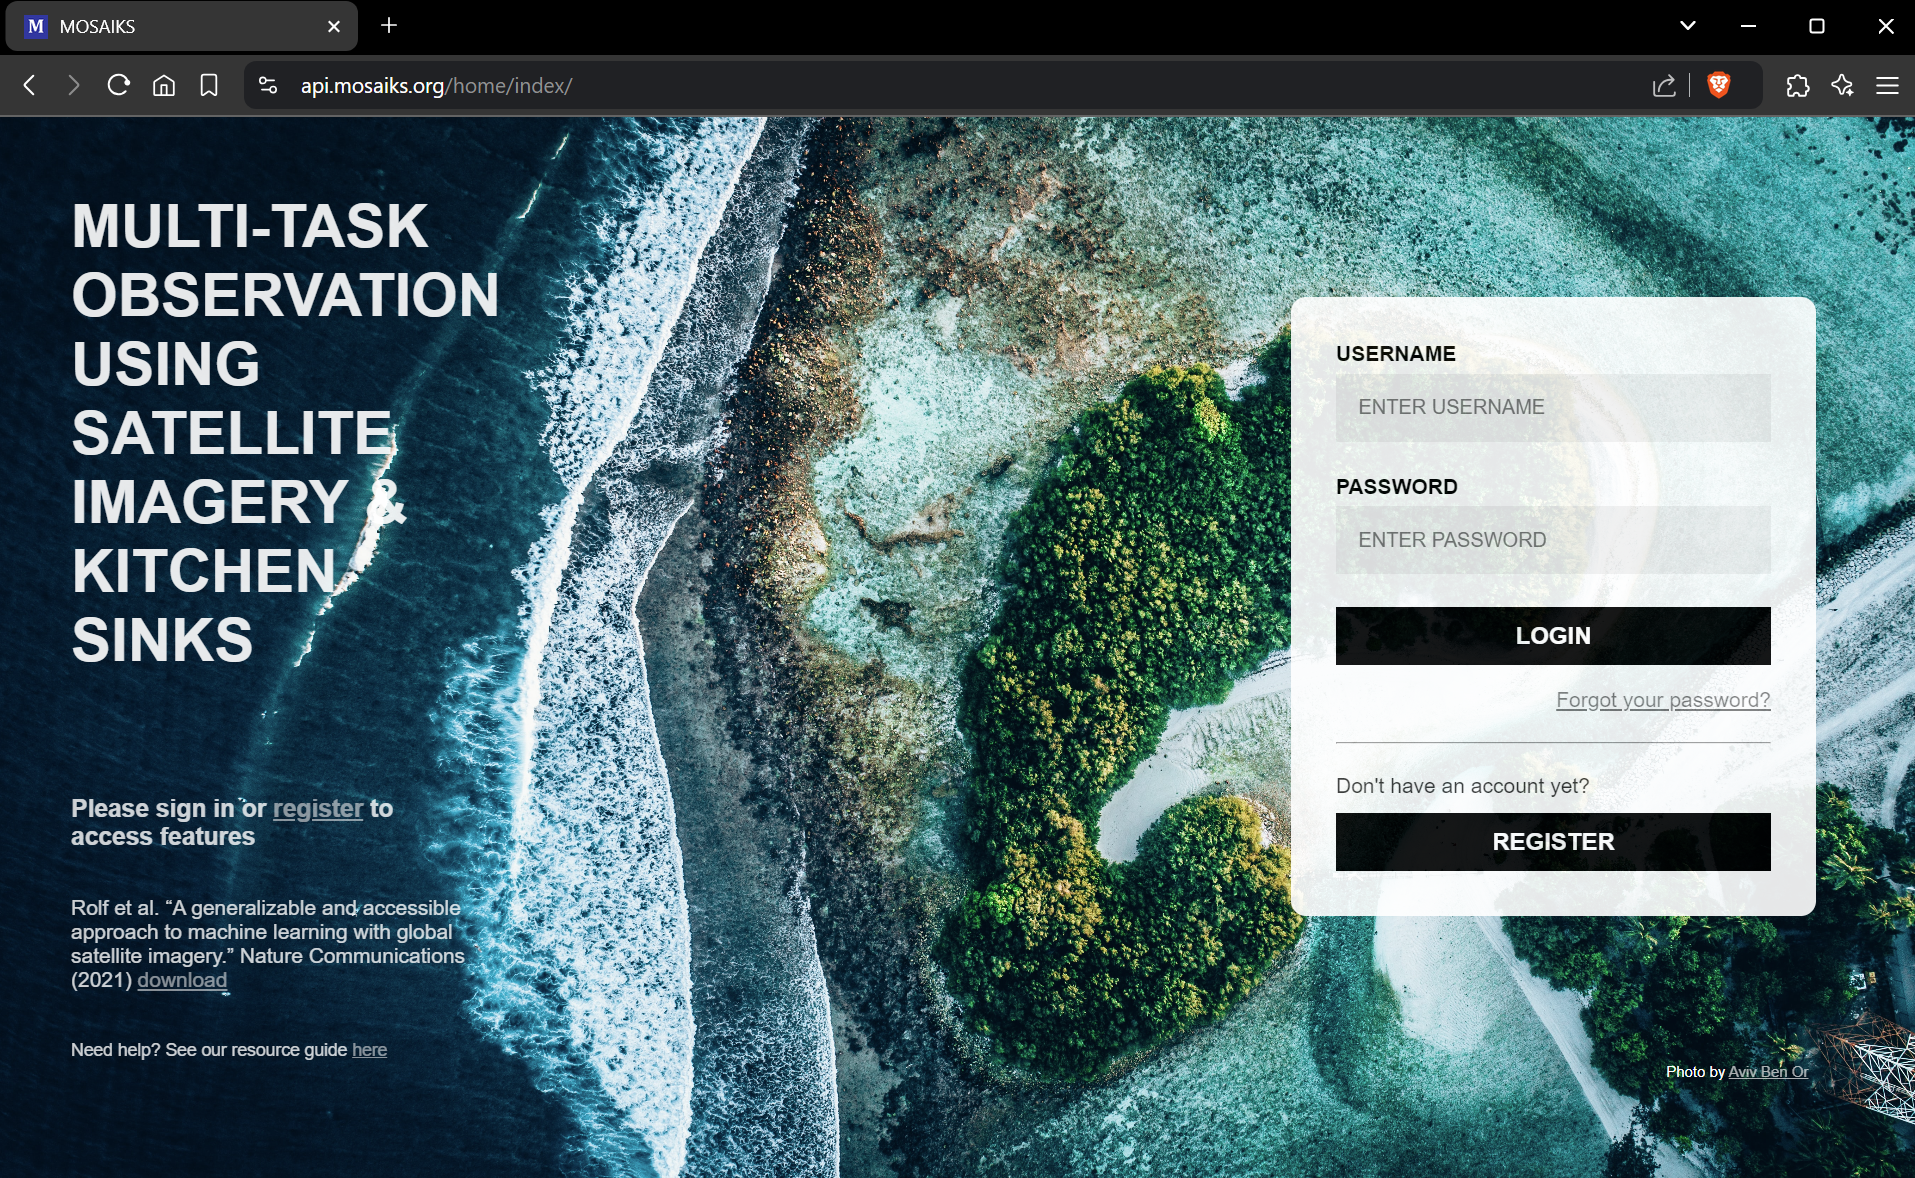
\includegraphics{images/api-home.png}

}

\caption{Landing page}

\end{figure}

Select \texttt{Register} to create an account. You'll need to provide:

\begin{figure}

{\centering \includegraphics{images/api-register.png}

}

\caption{Registration page}

\end{figure}

Once registered, you can log in to access the MOSAIKS features and begin
downloading data.

\begin{figure}

{\centering \includegraphics{images/api-landing.png}

}

\caption{Landing page}

\end{figure}

\hypertarget{downloading-features}{%
\section{Downloading features}\label{downloading-features}}

The MOSAIKS features are organized using a 0.01 x 0.01 degree
latitude-longitude global grid, centered at .005 degree intervals.

When you download features, you'll receive them in a tabular .csv format
where: - Each row represents a unique grid cell - The first two columns
contain latitude and longitude coordinates - The remaining columns
represent K features (currently K = 4000 features)

Important notes about downloads: - Files remain available for download
for 15 days - After 15 days, files are automatically deleted from the
system - There is a limit of 100,000 records per query

\hypertarget{ways-to-query-features}{%
\subsection{Ways to query features}\label{ways-to-query-features}}

There are two main methods to obtain features through the API:

\begin{enumerate}
\def\labelenumi{\arabic{enumi}.}
\tightlist
\item
  \textbf{Map Query}
\end{enumerate}

\begin{itemize}
\tightlist
\item
  Create rectangular boxes by specifying latitude and longitude
  coordinates
\item
  Multiple boxes can be created
\item
  The system displays an estimated number of records for each box
\item
  Note that estimates are based on box area and may not reflect actual
  record numbers, especially for areas containing seas and oceans
\end{itemize}

\begin{enumerate}
\def\labelenumi{\arabic{enumi}.}
\setcounter{enumi}{1}
\tightlist
\item
  \textbf{File Query}
\end{enumerate}

\begin{itemize}
\tightlist
\item
  Submit a file with custom latitude and longitude coordinates
\item
  The API returns features for grid cells closest to your input
  coordinates
\item
  Points are allocated to the nearest grid point if they don't exactly
  match
\item
  The output file may have a different number of rows than your input
\item
  Point ordering may change in the output
\end{itemize}

\begin{figure}

{\centering \includegraphics{images/api-map-n-file.png}

}

\caption{API Map Query (left) and File Query (right)}

\end{figure}

\hypertarget{using-mosaiks-features-for-prediction}{%
\section{Using MOSAIKS features for
prediction}\label{using-mosaiks-features-for-prediction}}

To use MOSAIKS effectively:

\begin{enumerate}
\def\labelenumi{\arabic{enumi}.}
\tightlist
\item
  Obtain ground truth measurements (``labels'') for your variable of
  interest
\item
  Download matching features using either Map Query or File Query
\item
  Perform a spatial merge between your labels and the features
\item
  Use regression to estimate the relationship between imagery features
  and your outcome variable
\end{enumerate}

You can experiment with various machine learning approaches in the
regression step. For beginners, we recommend starting with our example
Jupyter notebook that demonstrates a simple ridge regression approach
(suitable for both R and Python users).

This topic will be covered in greater depth in later chapters. In the
next chapter, you will see a simple MOSAIKS workflow which starts from
the point of having both features from the API and ground truth labels.

\hypertarget{citation-requirements}{%
\section{Citation requirements}\label{citation-requirements}}

When referring to the MOSAIKS methodology or when generating MOSAIKS
features, please reference
\href{https://www.nature.com/articles/s41467-021-24638-z}{Rolf et
al.~``A generalizable and accessible approach to machine learning with
global satellite imagery.'' Nature Communications (2021).}

You can use the following Bibtex:

\begin{Shaded}
\begin{Highlighting}[]
\VariableTok{@article}\NormalTok{\{}\OtherTok{article}\NormalTok{,}
    \DataTypeTok{author}\NormalTok{ = \{Rolf, Esther and Proctor, Jonathan and Carleton, Tamma and Bolliger, Ian and Shankar, Vaishaal and Ishihara, Miyabi and Recht, Benjamin and Hsiang, Solomon\},}
    \DataTypeTok{year}\NormalTok{ = \{2021\},}
    \DataTypeTok{month}\NormalTok{ = \{07\},}
    \DataTypeTok{pages}\NormalTok{ = \{\},}
    \DataTypeTok{title}\NormalTok{ = \{A generalizable and accessible approach to machine learning with global satellite imagery\},}
    \DataTypeTok{volume}\NormalTok{ = \{12\},}
    \DataTypeTok{journal}\NormalTok{ = \{Nature Communications\},}
    \DataTypeTok{doi}\NormalTok{ = \{10.1038/s41467{-}021{-}24638{-}z\}}
\NormalTok{\}}
\end{Highlighting}
\end{Shaded}

If using features downloaded from this website, please reference, in
addition to the publication above, the MOSAIKS API.

You can cite the API using the following Bibtex:

\begin{Shaded}
\begin{Highlighting}[]
\CommentTok{ }\VariableTok{@misc}\NormalTok{\{}\OtherTok{MOSAIKS} \OtherTok{API}\NormalTok{,}
    \DataTypeTok{author}\NormalTok{ = \{\{Carleton, Tamma and Chong, Trinetta and Druckenmiller, Hannah and Noda, Eugenio and Proctor, Jonathan and Rolf, Esther and Hsiang, Solomon\}\},}
    \DataTypeTok{title}\NormalTok{ = \{\{Multi{-}Task Observation Using Satellite Imagery and Kitchen Sinks (MOSAIKS) API\}\},}
    \DataTypeTok{howpublished}\NormalTok{ = "}\CharTok{\textbackslash{}url}\StringTok{\{ https://api.mosaiks.org \}}\NormalTok{",}
    \DataTypeTok{version}\NormalTok{ = \{1.0\},}
    \DataTypeTok{year}\NormalTok{ = \{2022\},}
\NormalTok{\}}
\end{Highlighting}
\end{Shaded}

\hypertarget{demonstration-of-mosaiks}{%
\chapter{Demonstration of MOSAIKS}\label{demonstration-of-mosaiks}}

\begin{itemize}
\tightlist
\item
  Description of exercise
\item
  Link to Google Colab Notebook
\item
  Video maybe?
\end{itemize}

\part{Label Data}

While MOSAIKS can involve many optional steps, its effective utilization
necessitates two core components:

\begin{enumerate}
\def\labelenumi{\arabic{enumi}.}
\tightlist
\item
  Ground observations (labels)
\item
  Satellite features
\end{enumerate}

Ensuring the spatial resolution is shared across both datasets and that
they contain geographical data suitable for merging is crucial.

\hypertarget{ground-observations}{%
\section*{Ground observations}\label{ground-observations}}
\addcontentsline{toc}{section}{Ground observations}

\markright{Ground observations}

The preparation of label data for MOSAIKS hinges on multiple factors,
particularly spatial information such as location, extent, and
resolution. If the observations in a dataset have a higher resolution
than 1 km², some form of selection or aggregation is required. Label
data can come in any native spatial form: raster, point, polygon, or
vector. As long as there is spatial information associated with each
label data observation, these data can be joined to MOSAIKS imagery
features for downstream prediction.

\begin{tcolorbox}[enhanced jigsaw, opacityback=0, left=2mm, leftrule=.75mm, colback=white, opacitybacktitle=0.6, colbacktitle=quarto-callout-note-color!10!white, toprule=.15mm, arc=.35mm, toptitle=1mm, colframe=quarto-callout-note-color-frame, bottomrule=.15mm, coltitle=black, bottomtitle=1mm, rightrule=.15mm, titlerule=0mm, title=\textcolor{quarto-callout-note-color}{\faInfo}\hspace{0.5em}{Note}, breakable]

The MOSAIKS API is designed to predict outcomes at scales of 1 km² or
larger. Customizable solutions are possible for higher resolution
problems..

\end{tcolorbox}

\begin{figure}

{\centering \includegraphics{images/rolf_et_al_2021-Fig_S4.png}

}

\caption{\label{fig-label-agg}Examples of label data formats that can be
easily integrated into the MOSAIKS pipeline. Label data of any spatial
format that can be aggregated to at least the scale of 1km2 (or larger)
can be used directly in combination with MOSAIKS imagery features for
downstream prediction tasks. Examples shown here are from Rolf et
al.~(2021) and include: forest cover, elevation, population, and
nighttime lights datasets (all raster format); income data (polygon
format); road length (vector format); and housing price data (point
format).}

\end{figure}

As with many machine learning algorithms, a large sample size often
results in higher performance than low. MOSAIKS has been used and shown
to be effective with a wide range of sample sizes (\emph{N}). The sample
size for model training is determined by the spatial and temporal
resolution of your label data. For example, when predicting maize yields
in the US using ground data from one year of farmer-level surveys in the
US, \emph{N}=3,143 if farmers are geolocated based on their county (even
if far more than 3,143 farmers were interviewed, as this is the number
of counties in the US). Additional time periods increase sample size for
training, but also require more up-front costs, as more imagery need to
be ``featurized''.

The original MOSAIKS publication (Rolf et al., 2021) tested performance
for forest cover, income, housing price, population density, nighttime
luminosity, and elevation using sample sizes ranging from 60,000 to
100,000, but showed that performance fell only modestly when N shrank to
just a few hundred observations. Consistent with this finding, in recent
experiments with crop yield, we see high with only around 400
observations (R2 = 0.80). It is important to note that the original crop
yield dataset included interview data from thousands of farmers across
the study country, and this messy data was cleaned and aggregated to the
district level prior to modeling. In this case, a clean dataset with a
low number of observations was preferred to a large but noisy dataset.
Despite the low sample size of the aggregate data, performance was still
comparable to more complex CNN models trained specifically on crop
yield.

MOSAIKS accommodates both continuous (e.g., fraction of area forested)
and discrete (e.g., presence/absence of water) labels, with data type
influencing model development and testing. Performance metric selection
is also determined by data type - for continuous variables, we typically
use the coefficient of determination (R²), while for discrete variables,
the area under the curve value from the receiver operator characteristic
curve (ROC AUC score) is used.

Currently the MOSAIKS API has a single global set of features that are
precalculated and ready to download. The features were computed from
satellite images from 2019 and are readily accessible to download and
use. Given this, the easiest way to get started with MOSAIKS is to have
label data for a recent time period (ideally from 2019 for fast changing
labels, or a close year for more steady labels). To use MOSAIKS for time
series data is possible, just not currently with precomputed and
publicly available features. The public MOSAIKS features available on
the API also have the advantage of being computed from cloud free, high
resolution images.

In sum, for ease of use with MOSAIKS, label data should:

\begin{itemize}
\tightlist
\item
  Be consistently geolocated as point, polygon, vector, or raster data\\
\item
  Be in a format that can be aggregated to at least 1km2, or lower
  resolution\\
\item
  Reflect an outcome that can feasibly be observed in daytime satellite
  imagery, or is the result or driver of an outcome that can feasibly be
  observed in daytime satellite imagery\\
\item
  Be relatively recent, if use with current MOSAIKS imagery features is
  desired\\
\item
  Be of at least size N=300, with expectations of higher performance at
  higher sample sizes
\end{itemize}

\hypertarget{feature-data}{%
\section*{Feature data}\label{feature-data}}
\addcontentsline{toc}{section}{Feature data}

\markright{Feature data}

\begin{tcolorbox}[enhanced jigsaw, opacityback=0, left=2mm, leftrule=.75mm, colback=white, opacitybacktitle=0.6, colbacktitle=quarto-callout-note-color!10!white, toprule=.15mm, arc=.35mm, toptitle=1mm, colframe=quarto-callout-note-color-frame, bottomrule=.15mm, coltitle=black, bottomtitle=1mm, rightrule=.15mm, titlerule=0mm, title=\textcolor{quarto-callout-note-color}{\faInfo}\hspace{0.5em}{Note}, breakable]

Processing satellite imagery and image featurization are covered in
later chapters.

\end{tcolorbox}

MOSAIKS relies on random convolutional features computed from satellite
imagery. The random nature of the features means that they are
task-agnostic. These features can be reused multiple times to model
various tasks. Features are generally created over a standard grid of
0.01 by 0.01 degree cells (\textasciitilde1 km2, depending on latitude),
although this can be customized in longer-term collaborations. The
output is a feature vector of length K for every location. Depending on
the spatial scale and resolution of the label data, subsampling the
MOSAIKS grid may be appropriate to reduce computation time and cost.

This 1 km resolution is generally the maximum resolution the label data
should be in. If the labels are in lower resolution, the satellite
features can be aggregated up to larger areas to match. Typical
aggregation might be to census tract, county/district, or state/province
levels. The exact aggregation level is contingent on the spatial
resolution of the label data.

The MOSAIKS API has 2019 Planet Labs, Inc.~imagery features publicly
available for download; this is the fastest and easiest way to begin
using MOSAIKS. However, satellite features can be created at varying
temporal scales. Publicly available satellite imagery such as Landsat
and Sentinel offer a rich time series, but their use with MOSAIKS will
require custom feature generation. The label data's timestep will play
an important role in determining the satellite imagery required for
computing features.

Data quality can also be affected by cloud cover. This may affect your
choice of satellite. For instance, if you require monthly features, the
slower revisit time of Landsat may mean many months will lack coverage
due to cloud cover limiting your ability to create high quality
features.

Another important part of picking the best imagery is the resolution of
the satellite sensor. This should be guided by intuition of what scale
is necessary for the satellite to detect your labels, as well as
availability of imagery. For example, tree cover may not require the
same resolution of imagery to detect effectively as crop yield.

The simplest implementation uses composite satellite images that are
highly processed to remove clouds and low quality pixels, and is often
normalized and color balanced. This is available directly on the MOSAIKS
API.

Processing satellite imagery and image featurization is covered in later
chapters.

\hypertarget{joining-data}{%
\section*{Joining data}\label{joining-data}}
\addcontentsline{toc}{section}{Joining data}

\markright{Joining data}

\textbf{Note:} Add example code

Before model training, label data must be joined to imagery features.
The joined data should be tabular with each row containing: 1.
Geographic location - such as a MOSAIKS grid cell or larger geographic
area 1. Label - the observed value 1. Time - an optional column useful
for time series data (year, mont, or day) 1. A column for every random
satellite feature (usually about 4,000 of these)

For example, a joined dataset could look like:

\begin{longtable}[]{@{}
  >{\raggedright\arraybackslash}p{(\columnwidth - 16\tabcolsep) * \real{0.1429}}
  >{\raggedright\arraybackslash}p{(\columnwidth - 16\tabcolsep) * \real{0.1209}}
  >{\raggedright\arraybackslash}p{(\columnwidth - 16\tabcolsep) * \real{0.0659}}
  >{\raggedright\arraybackslash}p{(\columnwidth - 16\tabcolsep) * \real{0.1319}}
  >{\raggedright\arraybackslash}p{(\columnwidth - 16\tabcolsep) * \real{0.1209}}
  >{\raggedright\arraybackslash}p{(\columnwidth - 16\tabcolsep) * \real{0.1209}}
  >{\raggedright\arraybackslash}p{(\columnwidth - 16\tabcolsep) * \real{0.1209}}
  >{\raggedright\arraybackslash}p{(\columnwidth - 16\tabcolsep) * \real{0.0549}}
  >{\raggedright\arraybackslash}p{(\columnwidth - 16\tabcolsep) * \real{0.1209}}@{}}
\toprule\noalign{}
\begin{minipage}[b]{\linewidth}\raggedright
Observation
\end{minipage} & \begin{minipage}[b]{\linewidth}\raggedright
District
\end{minipage} & \begin{minipage}[b]{\linewidth}\raggedright
Year
\end{minipage} & \begin{minipage}[b]{\linewidth}\raggedright
Crop Yield
\end{minipage} & \begin{minipage}[b]{\linewidth}\raggedright
Feature 1
\end{minipage} & \begin{minipage}[b]{\linewidth}\raggedright
Feature 2
\end{minipage} & \begin{minipage}[b]{\linewidth}\raggedright
Feature 3
\end{minipage} & \begin{minipage}[b]{\linewidth}\raggedright
\ldots{}
\end{minipage} & \begin{minipage}[b]{\linewidth}\raggedright
Feature K
\end{minipage} \\
\midrule\noalign{}
\endhead
\bottomrule\noalign{}
\endlastfoot
1 & Chibombo & 2016 & 1.520 & 4 & 11 & 15 & \ldots{} & 12 \\
2 & Kabwe & 2016 & 1.878 & 2 & 5 & 2 & \ldots{} & 11 \\
3 & Mkushi & 2016 & 2.078 & 3 & 8 & 3 & \ldots{} & 6 \\
4 & Mumbwa & 2016 & 1.923 & 5 & 4 & 9 & \ldots{} & 7 \\
5 & Serenje & 2016 & 1.180 & 2 & 7 & 14 & \ldots{} & 5 \\
6 & Chingola & 2016 & 2.566 & 1 & 0 & 12 & \ldots{} & 12 \\
\ldots{} & \ldots{} & \ldots{} & \ldots{} & \ldots{} & \ldots{} &
\ldots{} & \ldots{} & \ldots{} \\
N & Kitwe & 2022 & 2.383 & 10 & 1 & 6 & \ldots{} & 2 \\
\end{longtable}

In the above example, our geographic location is the district, our label
is the crop yield, and our time component is the year. We then have K
columns containing the features.

In this example, our features started at 1 km2 resolution and were
aggregated to the district level to match the crop yield data. To join
this data, we first found all of the feature locations that fall within
the district boundaries using a spatial join. Then we averaged the
features within each district. This allowed us to have a single feature
vector for each district. The resulting tabular data is then ready for
modeling.

\hypertarget{what-labels-work}{%
\chapter{What labels work?}\label{what-labels-work}}

\hypertarget{maps}{%
\section{100 Maps}\label{maps}}

\begin{itemize}
\tightlist
\item
  100 Maps results
\end{itemize}

\hypertarget{time-series-data}{%
\chapter{Time series data}\label{time-series-data}}

For time series data, the frequency of observation and rate of change
should also be considered when selecting satellite imagery to create
features. For instance, during a region's rainy season it may be much
more difficult to obtain high quality cloud free images. This has the
potential to leave large gaps in the feature data and may require
imputation to fill these gaps.

Take crop yield for example. The data is typically annual, but the
seasonal conditions can have a massive impact on yield. To capture
seasonal variation, monthly or quarterly satellite features can be used
with yearly labels. This would mean that each observation has K features
for each time step t (K*t features). Let's say we have 1,000 features
computed monthly, then our crop yield would be predicted by 12,000
features. An important point of this data is that there are consistent
locations with regular yield measurements.

\hypertarget{preparing-labels}{%
\chapter{Preparing labels}\label{preparing-labels}}

\begin{itemize}
\tightlist
\item
  Considerations for data cleaning
\item
  What should my data look like?
\end{itemize}

\hypertarget{demo-number-2}{%
\chapter{Demo Number 2}\label{demo-number-2}}

\begin{itemize}
\tightlist
\item
  IDK yet
\end{itemize}

\hypertarget{agriculture-example}{%
\chapter{Agriculture example}\label{agriculture-example}}

\part{Satellite Imagery}

\hypertarget{imagery-for-mosaiks}{%
\section*{Imagery for MOSAIKS}\label{imagery-for-mosaiks}}
\addcontentsline{toc}{section}{Imagery for MOSAIKS}

\markright{Imagery for MOSAIKS}

\hypertarget{overview-of-satellite-data}{%
\chapter{Overview of satellite data}\label{overview-of-satellite-data}}

\begin{itemize}
\tightlist
\item
  Spatial res
\item
  Temporal res
\end{itemize}

\hypertarget{public-satellites}{%
\chapter{Public Satellites}\label{public-satellites}}

\begin{itemize}
\tightlist
\item
  \href{https://sentinel.esa.int/web/sentinel/missions/sentinel-1}{Sentinel-1}
\item
  \href{https://sentinel.esa.int/web/sentinel/missions/sentinel-2}{Sentinel-2}
\item
  \href{https://www.usgs.gov/land-resources/nli/landsat/landsat-8}{Landsat
  8}
\item
  \href{https://modis.gsfc.nasa.gov/}{MODIS}
\item
  \href{https://www.ngdc.noaa.gov/eog/viirs/download_dnb_composites.html}{VIIRS}
\item
  \href{https://asterweb.jpl.nasa.gov/}{ASTER}
\end{itemize}

\hypertarget{private-satellites}{%
\chapter{Private Satellites}\label{private-satellites}}

\begin{itemize}
\tightlist
\item
  \href{https://www.maxar.com/products/satellite-imagery/worldview}{WorldView}
\item
  \href{https://www.planet.com/}{Planet}

  \begin{itemize}
  \tightlist
  \item
    \href{https://www.planet.com/products/skysat-imagery/}{SkySat}
  \item
    \href{https://www.planet.com/products/rapideye/}{RapidEye}
  \end{itemize}
\end{itemize}

\hypertarget{processing-satellite-data}{%
\chapter{Processing Satellite Data}\label{processing-satellite-data}}

\begin{itemize}
\tightlist
\item
  Download vs cloud processing
\end{itemize}

\part{Satellite Features}

\begin{itemize}
\tightlist
\item
  RCFs
\end{itemize}

\hypertarget{api-features}{%
\chapter{API Features}\label{api-features}}

\begin{itemize}
\tightlist
\item
  Defaults
\end{itemize}

\hypertarget{computing-features}{%
\chapter{Computing Features}\label{computing-features}}

\part{Task Modeling}

\hypertarget{model-choice}{%
\chapter{Model Choice}\label{model-choice}}

\hypertarget{filling-spatial-data-gaps}{%
\chapter{Filling spatial data gaps}\label{filling-spatial-data-gaps}}

\hypertarget{filling-temporal-data-gaps}{%
\chapter{Filling temporal data gaps}\label{filling-temporal-data-gaps}}

\part{Model Uncertainty}

\hypertarget{overview-of-uncertainty}{%
\chapter{Overview of uncertainty}\label{overview-of-uncertainty}}

\hypertarget{ethical-implications}{%
\chapter{Ethical implications}\label{ethical-implications}}

\bookmarksetup{startatroot}

\hypertarget{references}{%
\chapter*{References}\label{references}}
\addcontentsline{toc}{chapter}{References}

\markboth{References}{References}

\hypertarget{refs}{}
\begin{CSLReferences}{0}{0}
\end{CSLReferences}



\end{document}
